\documentclass[12pt]{article} 
\usepackage[brazil]{babel} %hifenização em português do brasil
\usepackage{gensymb}
\usepackage[pdftex]{hyperref}
\usepackage[T1]{fontenc} % caracteres com acentos são considerados um bloco só
\usepackage{graphicx}
\usepackage{ae} %arruma a fonte quando usa o pacote acima
\usepackage[utf8]{inputenc}
\usepackage{graphicx}%Para inserir figuras

\usepackage{cite}

\begin{document} % Aqui começa o documento
\title{Implementação \textit{system calls} no kernel linux V. 4.13.12\vspace{3.5cm}} % título

\author{
	João Paulo de Oliveira
	\texttt{joaopaulodeoliveira123@gmail.com}
	\and
	Lucas Rossi Rabelo
	\texttt{lucasrossi98@hotmail.com}
	\and		
	Matheus Pimenta Reis
	\texttt{matheu}
	\vspace*{9cm}
}

\maketitle
\tableofcontents

\pagebreak
\section*{Implementação \textbf{System Calls} no Linux}
As \textit{System Calls} fazer o interfaceamento entre o hardware e os processo do espaço de usuário, elas também servem para três propósitos principais:
\begin{enumerate}
	\item Provém abstração com o hardware para que o usuário tenha um maior rendimento. Por exemplo, o usuário não se preocupa com o tipo de partição em que ele lerá um arquivo;
	\item As \textit{system calls} garantem a segurança e estabilidade para que um usuário relativamente leigo possa ter um alto rendimento com gerência de permissão, usuários e outros critérios de gerência do kernel;
	\item Uma camada entre espaço de usuário e o resto do sistema permite fornece o sistema virtualizado para os processos.
\end{enumerate}
	As chamadas syscalls em linux são, na maioria dos casos, acessadas pelas funções definidas na C library. As syscalls em si retornam um valor do tipo long4 que, quando negativo, em geral, denota um erro, já o retorno com valor zero (nem sempre) é um sinal de sucesso. A C library, quando uma \textit{system call} retorna um erro, ela grava o código desse erro na variável global errno, que pode ser ser traduzida para um texto que fala sobre o erro através de funções de biblioteca.
	
	Para a implementação de uma \textit{system call} deve-se ter acesso ao código do kernel do sistema operacional para tanto, foi escolhido o kernel Linux que é open source.
\subsection*{Download do Kernel}
Por ser open source, o código fonte do kernel do Linux é mantido online para livre acesso no GitHub(\url{https://github.com/torvalds/linux}), e também em The Linux Kernel Archives (\url{https://www.kernel.org/}) em várias versões e formatos de arquivos(compactados). A versão mais recente dado a data de início do TCD foi a versão \textbf{14.13.12}.
de gerência do kernel.
	A Free Software Foundation mantém, gerencia e presta suporte para o The Linux Kernel Archives.O donwnload do kernel pode ser feito facilmente, além de outras funções com perguntas frequentes, download de versões em teste (beta) para ser compilado em qualquer distribuição linux ou em outras plataformas que suportam o kernel.
	\vspace*{2cm}
	 Como pode ser visto na imagem abaixo:
\begin{figure}[!h]
	\centering
	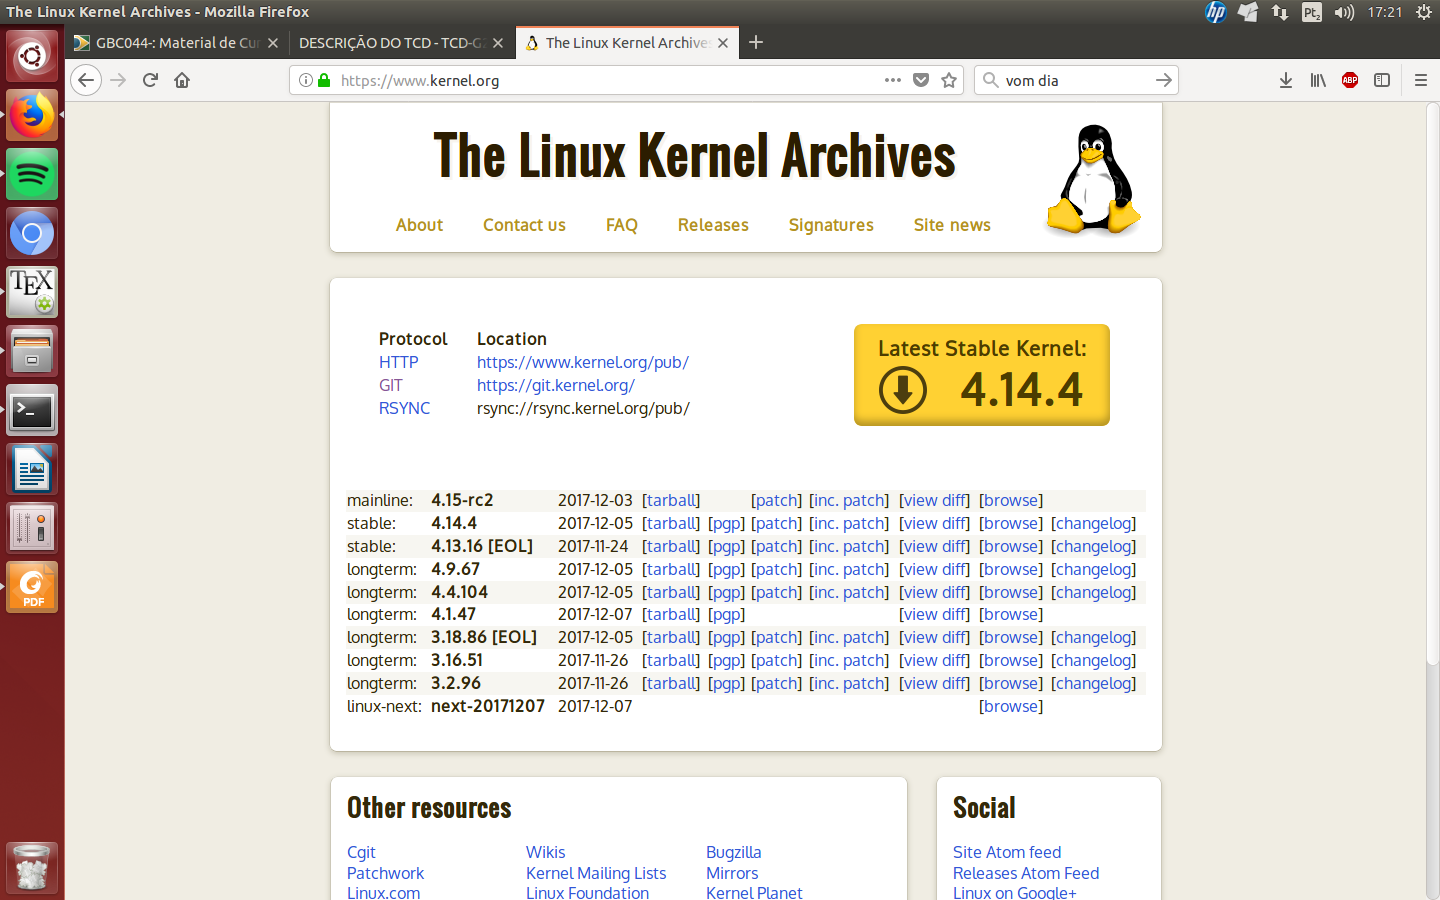
\includegraphics[scale=0.2]{imagens/kernelorg.png}
	\caption{The Linux Kernel Archives: Local de download do Kernel}
	\label{kernelorg}
\end{figure}
\subsection*{Criação da System Call}
A \textit{system call} foi criada dentro na pasta kernel no diretório principal deixando o arquivo  scall.c nessa pasta. Após isso foi adicionado o arquivo objeto no arquivo de \textit{makefile} como descrito no tutorial, dessa forma, foi encontrada no arquivo \textit{syscall\_64.tbl} na forma: \newline

\textbf{333	common	scall			sys\_det}
\newline
Assim a função pode ser chamada pela função \textit{\textbf{syscall(333)}} presente na \textit{unistd.h}. Por fim, foi adicionado o cabeçalho da função no arquivo \textit{syscall.h}. Depois disso foi compilado o kernel seguindo o tutorial proposto  %\cite{tutorial}. 
\\ \newline
\scriptsize{\textbf{unsigned long copy\_to\_user(void \_user *to, const void *from, unsigned long n)};}
\newline
	
Vejamos agora o código do kernel utilizado para

\subsubsection*{Tempo na CPU}
Como primeira tentativa para obter o tempo de CPU de um processo, acessamos a variável \textit{sum\_exec\_runtime} na estrutura \textit{task\_cputime}, com base nos comentários da estrutura, concluímos que tal variável era o que desejávamos como segue na figura 2: %fazer um hiperlink

\begin{figure}[!h]
	\centering
	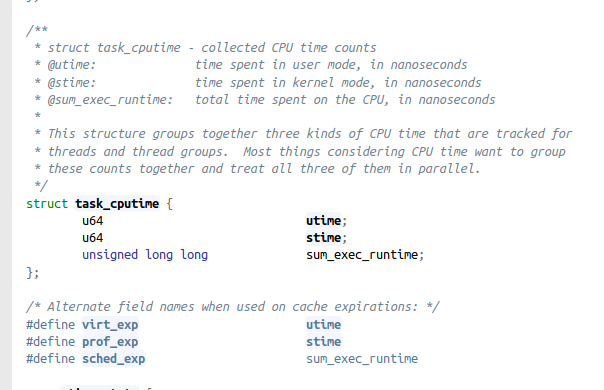
\includegraphics[scale=0.5]{imagens/img1.png}
	\caption{Estrutura task\_cputime}
	\label{taskcputime}
\end{figure}

No entanto, com a tentativa não obtivemos o resultado esperado.
Como segunda tentativa, encontramos uma outra estrutura chamada \textit{sched\_entity} na qual, na mesma, encontra-se uma outra variável chamada \textit{sum\_exec\_runtime}, como segue na imagem abaixo:

\begin{figure}[!htb]
	\centering
	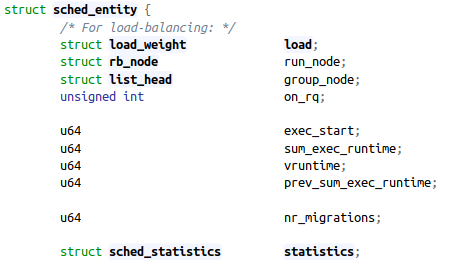
\includegraphics[scale=0.4]{imagens/img2.png}
	\caption{Parte da estrutura sched\_entity}
	\label{schedentity}
\end{figure}

Depois procuramos na \textit{task\_struct} a declaração de uma variável do tipo \textit{sched\_entity}:

\begin{figure}[!htb]
	\centering
	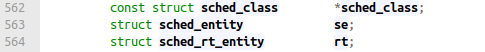
\includegraphics[scale=0.8]{imagens/img3.png}
	\caption{Declaração da sched\_entity na linha 563 na task\_struct}
	\label{decschedentity}
\end{figure}




\subsubsection*{Tempo de vida do processo}
\subsubsection*{N$^{\circ}$  de vezes que o processo passou pela CPU}
\subsection*{Código da system call}
Foi usada também a função copy\_to\_user para copiar um bloco de dados do kernel para o espaço de usuário para que a função possa retornar por parâmetro

\subsection*{Programa usuário da system call}




\bibliographystyle{abbrv}
\bibliography{refs}
\end{document}
